% !TEX program = pdflatex
% arXiv preprint (English). Build: pdflatex main && bibtex main && pdflatex main (x2)
% If your TeX distribution lacks newtx, replace it with:
%   \usepackage{times}
%   \usepackage{amsmath,amsfonts}
\documentclass[11pt]{article}

\usepackage[margin=1in]{geometry}
\usepackage[T1]{fontenc}
\usepackage{amsmath}
\usepackage{amsfonts}
\usepackage{newtxtext,newtxmath}   % Times-like text + math (standard on arXiv/Overleaf)
\usepackage{booktabs}
\usepackage{graphicx}
\usepackage{algorithm}
\usepackage{algpseudocode}
\usepackage{microtype}
\usepackage[hidelinks]{hyperref}
\usepackage{natbib}

\renewcommand{\algorithmicrequire}{\textbf{Input:}}
\renewcommand{\algorithmicensure}{\textbf{Output:}}
\setlength{\emergencystretch}{2em}

\graphicspath{{../figs/}}
\bibliographystyle{plainnat}

\title{Purpose-Driven Associative Retrieval:\\
Building a User-Modeling Context from a Memory Graph}

\author{Siyu Chen\thanks{Preprint v0.5.1: \url{https://doi.org/10.5281/zenodo.24373015}.
  Code, data, and evaluation scripts: \url{https://doi.org/10.5281/zenodo.24373025}.} \\
  Independent Researcher \\
  China \\
  \texttt{1405921723@qq.com}}
\date{November 2026}

\hypersetup{
  pdftitle={Purpose-Driven Associative Retrieval: Building a User-Modeling Context from a Memory Graph},
  pdfauthor={Siyu Chen}
}

\begin{document}
\maketitle

\begin{abstract}
Retrieval research mostly targets question answering: given a query, return passages that
contain the answer. Dialogue memory poses a different problem. The system must reconstruct
\emph{the user at this moment}---their state, preferences, relationships, constraints, and
history---rather than locate a passage. This task has no stable golden set: the same memory
may be relevant under one intent and irrelevant under another, so P@K and R@all cannot define
``correct'' or compare systems that build context differently.

We present \textbf{PAR} (Purpose-driven Associative Retrieval), a set-valued retrieval
mechanism over a typed memory graph. PAR expands candidates along typed relations with a
direction-aware weight matrix, scores them by purpose relevance (with a threshold that is
effectively inactive at the default 0.30), and stops by
a peak-tolerance band over round-level mean scores instead of a fixed hop count or top-$k$.
We evaluate the produced context blocks, not a ranked list, using three LLM judges on a
three-dimensional rubric.

On a 163-node emotional-companion memory graph with 76 queries, the full system scores
4.46--4.72 against 3.25--3.77 and 2.92--3.46 for two baselines, consistently ranked first by
all judges. In an isolated setting that fixes the graph and the assembler and changes only the
memory-selection mechanism, the full PAR+story configuration improves over vector top-$k$ by
1.35--1.86 on 70 non-abstention queries (the selection-only variant by 1.28--1.43), with a
rank-biserial correlation near 1.00. We also report a negative result that constrains the
claim: the purpose channel changes the retrieved set substantially (node-set Jaccard 0.31),
yet its direction is right about half the time, because a purpose represented as a pooled
embedding of abstract phrases carries topic but not ``what kind of content''. Rewriting the
purpose as three explicit requirements (content type, relation type, and episode) raises the
type-distribution divergence between intents from 0.09 to 0.47 at its natural output size
(0.29--0.36 at equal size) and gold-facet recall from 0.30 to 0.53, but those requirements are
still supplied by a hand-written mapping. We further
show that the default purpose-filter threshold of 0.30 removes no candidate on this graph; the
negative result therefore concerns purpose seeding and weighting, not filtering. The filter only
starts to bite at 0.45--0.55, where it trades output size for precision.
\end{abstract}

\section{Introduction}

\paragraph{From answering questions to modeling users.}
A typical RAG pipeline assumes that (i) a relatively stable set of relevant passages exists and
(ii) that set can be ranked by relevance and truncated at top-$k$. Dialogue memory violates
both assumptions. When the user says ``I have been really tired this week,'' the system does
not need a medical definition of fatigue. It needs to recall that the user has worked late for
several days, that a delivery is due on Friday, that they go to a caf\'e when stressed, and
that they dislike being told to ``just sleep earlier.'' These memories are not related to the
utterance by semantic similarity; they are related by the current \emph{purpose}.

The same memory can also be valuable under one intent and irrelevant under another. For the
utterance above, a user who wants to vent needs emotions and their causes; a user who wants to
plan needs next week's time anchors and tasks; a user who wants advice needs options and
past solutions that worked. We therefore treat dialogue-memory retrieval as
\emph{user-modeling retrieval}: given dialogue history, the current utterance, and a memory
graph, produce a set of memories that supports understanding the user at this moment.

\paragraph{Why P@K and R@all do not apply.}
Porting RAG metrics to this setting fails for three reasons. First, the ranking assumption does
not hold: PAR returns a set, and forcing it into a single-score order degenerates it into the
vector search it tries to avoid. Second, the golden-set assumption does not hold: relevance
depends on intent, so a fixed expected set can encode only one reading. Third, output size is
not comparable: R@all rewards systems that return more items, so a comparison between PAR's
6--27 nodes and a fixed 5-passage baseline mostly reflects the output budget.

We therefore do not use P@K or R@all as the main metric. Retrieval-side numbers appear only in
the appendix, as mechanism diagnostics. The main evaluation asks whether the produced context
block supports user modeling, scored by LLM judges under a fixed rubric.

\paragraph{Contributions.}
\begin{enumerate}
  \item \textbf{Problem formulation.} We separate question-answering retrieval from
        user-modeling retrieval, and formalize intent-conditioned relevance and set-valued
        retrieval.
  \item \textbf{Method.} PAR combines a direction-aware typed expansion (the \emph{jump axis}),
        purpose-based filtering, and a peak-tolerance stopping rule; its output is a set.
  \item \textbf{Evaluation protocol.} We replace a fixed golden set with multi-judge scoring of
        end-to-end context blocks, and report judge agreement and anonymization controls.
  \item \textbf{Evidence and boundaries.} A same-graph isolation experiment establishes the
        benefit of the selection mechanism ($r\approx1.00$). Product-level probes locate the
        purpose representation as the current bottleneck, give an acceptance criterion for
        improving it, and include a minimal working demonstration.
\end{enumerate}

\section{Related Work}

\paragraph{RAG and GraphRAG.}
Retrieval-augmented generation (RAG) decouples retrieval from generation and grounds outputs
in external documents \citep{lewis2020rag}. GraphRAG organizes a corpus into an entity--relation
graph and supplies context through community summaries or graph traversal
\citep{edge2024graphrag}; HippoRAG uses a knowledge graph with personalized PageRank to mimic
associative memory \citep{gutierrez2024hipporag}. These lines share one premise: the retrieval
target is a document or fact related to the query or the answer. PAR does not search for
answer evidence; it builds a model of the current user, so both the object being evaluated and
the optimization target differ.

\paragraph{Agent memory.}
Systems such as Mem0 and Zep/Graphiti persist conversations as memory units or as a temporal
knowledge graph, with emphasis on writing, updating, retrieving, and time validity
\citep{chhikara2025mem0,rasmussen2025zep}. They are usually evaluated by QA accuracy, retrieval
hits, or token cost. PAR is complementary in engineering terms: it asks how to take a set of
memories relevant to the current purpose out of an existing graph, not how to maintain the
memory store. Our end-to-end comparison therefore treats Mem0 and Graphiti as alternative
context builders rather than as retrieval baselines.

\paragraph{Associative memory and spreading activation.}
Spreading activation provides a cognitive account of how relevance propagates along relational
paths \citep{anderson1983spreading}. A growing line of recent systems combines spreading
activation with lateral inhibition and temporal decay, Hebbian learning with dual-path retrieval,
or associative graphs with active reconstruction or self-evolution. What PAR shares with them is
the refusal to equate relevance with vector similarity. It differs in four ways:

\begin{itemize}
  \item a typed weight matrix over \textbf{6 node types $\times$ 8 relation types $\times$
        direction}, where a zero weight acts as a structural block;
  \item the purpose is an \textbf{independent filter}, not merely a factor folded into edge
        weights;
  \item the output set is decided by a \textbf{peak-tolerance band over round-level purpose
        scores}, instead of a fixed hop count or top-$k$;
  \item the object being evaluated is a \textbf{user-modeling context}, not an answer or a
        ranked list.
\end{itemize}

\paragraph{Evaluating generated context.}
LLM-as-a-judge is established for generation quality, summarization, and dialogue
\citep{zheng2023judging}. We apply it to the context block rather than to the reply: the reply
model is decoupled so that conversational ability is not credited to the memory system, and
judge bias is controlled by side-by-side presentation, cross-model agreement, anonymization,
and repeated scoring. This asks whether the memory system supplied good material for user
modeling, not whether a model can chat.

\section{Problem Definition}

\subsection{Dialogue Memory and User Modeling}

Let $H$ be the dialogue history, $q$ the current utterance, and $G=(V,E)$ a memory graph. The
system must return a context set $R\subseteq V$ such that a downstream model reading $R$ can
better understand the user's current state, preferences, relationships, constraints, and
history. This differs from question-answering retrieval: there the goal is evidence that
supports an answer; here it is memories that support understanding the user. The two can
overlap, but they are not the same objective.

\subsection{Intent-Conditioned Relevance}

The relevance of a memory is not a fixed property. It is a function of the memory, the current
utterance, and the conversation state. Consider the memory ``the user has worked late for
several days'':

\begin{itemize}
  \item when the user says ``I am exhausted today,'' it is the key to empathy and to the cause;
  \item when the user says ``plan my weekend,'' it is a constraint and a preference cue;
  \item when the user says ``recommend a film,'' it may be entirely irrelevant.
\end{itemize}

We therefore do not define a fixed expected set. We define \emph{intent-conditioned relevance}:
given the current purpose $p=\phi(q)$, a memory $v$ is relevant if it serves $p$. Here $p$ is
not a paraphrase of the query but a representation of what the user wants to do, or how the
user wants to be understood, at this moment.

\subsection{Set-Valued Retrieval}

PAR returns a set,
\begin{equation}
  R=\mathrm{PAR}(G,q),
\end{equation}
not a ranked list. Elements of $R$ carry no promise of a total order; downstream components may
consume them in any way. The reason is that user modeling needs a set of material covering
several facets, not the five most similar memories. A list of five highly similar memories can
miss a cross-domain memory that is relevant to the intent but not semantically close to the
utterance.

\subsection{Evaluation Objective}

What we care about is
\begin{equation}
  \mathcal{U}(R,q)=\text{the usefulness of }R\text{ for modeling the current user}.
\end{equation}
$\mathcal{U}$ cannot be computed from a golden set, because it depends on the dialogue intent
and on the user's state. We approximate it with an LLM judge $J(R,q)$ and give the rubric and
reliability controls in Section~5. The optimization target of PAR is not to make $R$ hit a
list, but to make $J(R,q)$ higher.

\section{Method: PAR}

\subsection{Graph and Types}
\label{sec:graph}

In the memory graph $G=(V,E)$, every node carries a semantic role out of six types
(Table~\ref{tab:nodetypes}), and every directed edge carries one of eight relation types
(Table~\ref{tab:reltypes}). The typing is produced by the extraction pipeline and is not
re-estimated here; PAR only consumes it.

\begin{table}[t]
  \centering
  \small
  \begin{tabular}{@{}ll@{}}
    \toprule
    Node type & Meaning \\
    \midrule
    STATUS  & current state of the user or assistant \\
    REASON  & cause of a state or event \\
    ACTION  & something done or planned \\
    THING   & object, place, time, artifact \\
    PERSON  & people and relationships \\
    EMOTION & feelings \\
    \bottomrule
  \end{tabular}
  \caption{Node types.}\label{tab:nodetypes}
\end{table}

\begin{table}[t]
  \centering
  \small
  \begin{tabular}{@{}lll@{}}
    \toprule
    Relation & Meaning & Direction \\
    \midrule
    CAUSAL     & cause & to the result \\
    SCENARIO   & scenario membership & both \\
    SEQUENCE   & temporal order & to the successor \\
    PREFERENCE & attitude toward an object & to the object \\
    SOCIAL     & social tie & both \\
    ATTRIBUTE  & property of an entity & both \\
    TEMPORAL   & time anchoring & to the time \\
    TAXONOMIC  & taxonomy & to the parent \\
    \bottomrule
  \end{tabular}
  \caption{Relation types.}\label{tab:reltypes}
\end{table}

Graph construction and maintenance are outside the scope of this paper. The main experiments use a
manually built graph; the automatic graph in \S\ref{sec:e3} is produced by the DBA pipeline
summarised in Appendix~\ref{app:dba}. This paper treats the graph as an input and only varies its
source in \S\ref{sec:e3}; extraction-level quality is reported in Appendix~\ref{app:dba} and
is not used as a retrieval result.

\subsection{The Jump Axis}

PAR does not diffuse over all edges with a single coefficient. It defines a weight for each
triple of node type, relation type, and direction, i.e.\ a tensor
$W\in\mathbb{R}^{6\times 8\times 2}$. Table~\ref{tab:jumpaxis} shows the values used in this
paper; each cell reads forward/reverse, and $0$ means the direction is blocked rather than
merely down-weighted.

\begin{table}[t]
  \centering
  \footnotesize
  \setlength{\tabcolsep}{3pt}
  \begin{tabular}{@{}lcccccccc@{}}
    \toprule
    From & CAUSAL & SCENARIO & SEQUENCE & PREFERENCE & SOCIAL & ATTRIBUTE & TEMPORAL & TAXONOMIC \\
    \midrule
    STATUS  & 0.9/1.0 & 0.8/0.8 & 0.7/0.0 & 0.4/0.0 & 0.5/0.5 & 0.3/0.3 & 0.3/0.0 & 0.0/0.0 \\
    REASON  & 1.0/0.9 & 0.6/0.6 & 0.8/0.0 & 0.2/0.0 & 0.4/0.4 & 0.3/0.3 & 0.3/0.0 & 0.0/0.0 \\
    ACTION  & 0.9/0.7 & 0.8/0.8 & 0.9/0.6 & 0.5/0.0 & 0.6/0.6 & 0.4/0.4 & 0.5/0.0 & 0.0/0.3 \\
    THING   & 0.3/0.3 & 1.0/1.0 & 0.4/0.4 & 0.8/0.0 & 0.3/0.3 & 0.7/0.7 & 0.3/0.0 & 0.0/0.3 \\
    PERSON  & 0.5/0.5 & 0.6/0.6 & 0.5/0.5 & 0.8/0.0 & 1.0/1.0 & 0.7/0.7 & 0.4/0.0 & 0.0/0.0 \\
    EMOTION & 0.9/1.0 & 0.8/0.8 & 0.6/0.0 & 0.5/0.0 & 0.5/0.5 & 0.4/0.4 & 0.3/0.0 & 0.0/0.0 \\
    \bottomrule
  \end{tabular}
  \caption{Jump-axis weights (forward/reverse; $0$ blocks expansion).}\label{tab:jumpaxis}
\end{table}

Three principles governed the design. First, \emph{direction depends on the origin}: from a
STATUS node the useful move is toward the cause (reverse CAUSAL $=1.0$), the scenario, or the
subsequent behavior (forward CAUSAL $=0.9$), not toward an abstract parent (forward TAXONOMIC
$=0.0$). Second, \emph{a zero weight is a structural block}, not a small number: an emotional
query should not drift into unrelated categories through the taxonomy chain. Third, the matrix
encodes ordinal preferences (CAUSAL $>$ SCENARIO $>$ SEQUENCE) rather than fitted values. It is
a hand-specified prior, and Section~8 treats this as a limitation.

\subsection{Purpose Regression}

PAR first asks an LLM to extract one or two purpose phrases from the query and maps them to a
purpose embedding $e_p$. The purpose is not a paraphrase of the query; it abstracts what the
user wants to do, or how the user wants to be understood. A candidate $v$ enters the output
only if $\cos(e_v,e_p)\ge\tau_p$, with $\tau_p=0.30$ by default. The value is bound to the
embedding model and must be re-calibrated when the model changes (Section~7.3).

The purpose has two roles: it \emph{filters} semantic neighbours that are unrelated to the
current intent, and it \emph{orders} the candidates that survive, replacing query-to-node
cosine as the global ranking signal.

This design rests on an assumption: that the purpose can be represented as ``what kind of
content is wanted.'' The default representation is the pooled embedding of purpose phrases.
That representation keeps the topic but discards the requested content type, which is why the
channel is weak in practice (Section~6.6). We therefore also evaluate a structured
variant: the purpose is written as three requirements, namely the target node type, the
expected relation type, and the episode the user is talking about. The purpose score becomes a
multiplicative gate,
\begin{equation}
  s(v)=\cos(e_v,e_p)\cdot\bigl(\beta_0+\beta_t\,a_{\mathrm{type}}(v)
  +\beta_r\,a_{\mathrm{rel}}(v)\bigr),
\end{equation}
with $(\beta_0,\beta_t,\beta_r)=(0.55,0.35,0.10)$; $a_{\mathrm{type}}$ and $a_{\mathrm{rel}}$
are affinities in $[0,1]$ derived from the frame, with a floor of $0.25$ and $0.15$ so that
cross-type evidence is not cut off. The gate can modulate a candidate but cannot outvote topic
similarity. Figure~\ref{fig:mechanism} contrasts the pooled representation with the gated one.
The structured variant is opt-in and off by default; Section~6.10 reports what it changes.

\subsection{Peak-Tolerance Band}

PAR uses neither a fixed hop count nor a fixed top-$k$. At every round it computes the mean
purpose score of the survivors,
\begin{equation}
  \mu_h=\frac{1}{|F_h|}\sum_{v\in F_h}\cos(e_v,e_p),
\end{equation}
where $F_h$ is the set of candidates that passed the purpose filter at round $h$. The mean uses
purpose scores only. The combined score includes a hop-dependent decay, so using it for peak
detection would produce a spurious peak at the first hop.

Let $h^\ast=\arg\max_h\mu_h$. PAR collects every round with
$\mu_h\ge\mu_{h^\ast}-\delta$ ($\delta=0.10$ by default) and outputs the union of those rounds
after deduplication. This keeps multi-hop candidates near the peak instead of taking a single
round. The seed round is always included and is excluded from the peak sequence: its mean is
computed over the $k$ nodes closest to the query, a different population from the expansion
candidates, and including it would pin $h^\ast$ at zero.

\subsection{Algorithm}

Algorithm~\ref{alg:par} summarizes one retrieval. Step~2 only finds entry points; it does not
define the final order. The combined score in step~8 is used for ranking candidates within a
round, never for peak detection.

\begin{algorithm}[t]
  \caption{PAR}\label{alg:par}
  \begin{algorithmic}[1]
    \Require query $q$, graph $G=(V,E)$, weights $W$, seed size $k$, threshold $\tau_p$,
             hop limit $H$, band width $\delta$, patience
    \Ensure memory set $R$
    \State $p\gets\mathrm{InferPurpose}(q)$;\quad $e_p\gets\mathrm{Embed}(p)$
    \State $M_0\gets\mathrm{TopK}(q,k)$ \Comment{entry points only}
    \State $R\gets M_0$;\quad $S\gets M_0$;\quad $\mu^\ast\gets-\infty$;\quad $h^\ast\gets0$
    \For{$h=1$ \textbf{to} $H$}
      \State $C_h\gets\mathrm{Expand}(M_{h-1},W)\setminus S$
      \State $F_h\gets\{\,v\in C_h:\cos(e_v,e_p)\ge\tau_p\,\}$
      \If{$|F_h|=0$} \State \textbf{break} \EndIf
      \State $s_v\gets\alpha\,\mathrm{jw}(u\!\to\!v)\,\gamma^{\,h-1}
             +\beta\cos(e_v,e_p)$ \textbf{for} $v\in F_h$
      \State $\mu_h\gets\frac{1}{|F_h|}\sum_{v\in F_h}\cos(e_v,e_p)$
      \If{$\mu_h>\mu^\ast$} \State $\mu^\ast\gets\mu_h$;\quad $h^\ast\gets h$ \EndIf
      \If{$h-h^\ast>\text{patience}$} \State \textbf{break} \EndIf
      \State $R\gets R\cup F_h$;\quad $S\gets S\cup F_h$
    \EndFor
    \State \Return $\mathrm{dedupe}\bigl(M_0\cup\bigcup_{h:\,\mu_h\ge\mu^\ast-\delta}F_h\bigr)$
  \end{algorithmic}
\end{algorithm}

\subsection{Complexity}

Seed search costs $O(|V|\,d)$ (near-linear with an ANN index). Graph expansion costs
$O(\sum_h|E_h|)$; purpose filtering costs $O(\sum_h|C_h|\,d)$; ranking costs
$O(\sum_h|C_h|\log|C_h|)$. There is usually one LLM call for purpose inference (plus one for
state inference when it is decoupled). The dominant cost is therefore LLM inference and
embedding, not graph traversal.

\subsection{Relation to RAG and GraphRAG}

\begin{table}[t]
  \centering
  \small
  \begin{tabular}{@{}lll@{}}
    \toprule
    Dimension & RAG / GraphRAG & PAR \\
    \midrule
    Goal & evidence that supports an answer & a local model of the current user \\
    Output & ranked list / top-$k$ & set, with no total order promised \\
    Relevance & similarity to the query or answer & service to the current purpose \\
    Stopping & fixed $K$ or fixed hops & peak-tolerance band over purpose scores \\
    Evaluation & P@K, R@all, QA accuracy & LLM-judged context quality \\
    \bottomrule
  \end{tabular}
  \caption{PAR is not a stronger RAG; it answers a different question.}\label{tab:compare}
\end{table}

Table~\ref{tab:compare} states the difference compactly. PAR is not a stronger retriever for
answer evidence; it targets a different objective, and consequently a different evaluation
object.

\begin{figure}[t]
  \centering
  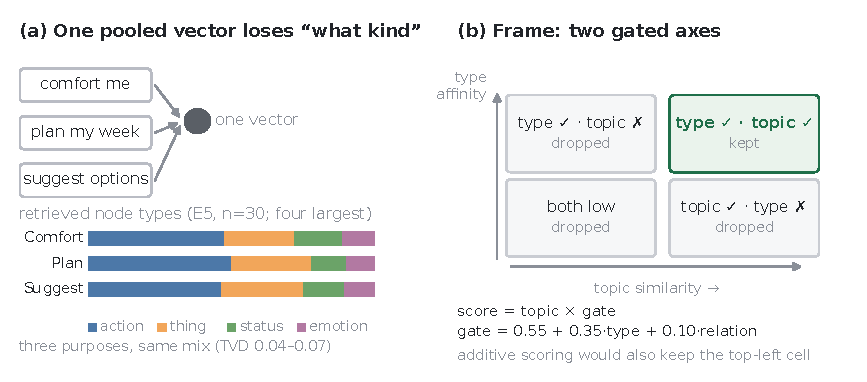
\includegraphics[width=\linewidth]{fig1_mechanism.pdf}
  \caption{(a) Pooling three purposes into one vector leaves the retrieved node-type mix almost
  identical across intents (E5, $n=30$; the four largest types are renormalised). (b) With three
  explicit requirements, only candidates that match both topic and type survive; additive
  scoring would also keep the top-left cell.}
  \label{fig:mechanism}
\end{figure}

\section{Evaluation Protocol}
\label{sec:protocol}

\paragraph{A note on metrics.}
We are not opposed to quantification; we require that a metric (i) measures what it claims to
measure, (ii) corresponds to behaviour that matters in use, and (iii) is stable enough that its
noise is smaller than the effect being claimed. Metrics borrowed from RAG---P@K, R@all,
recall@$k$, NDCG---encode three assumptions: a stable relevant set, a meaningful total order,
and comparable output budgets. Where any of the three fails, the metric is used only as a
mechanism diagnostic and never as a ranking of systems or as the sole basis for a claim. Every
comparison reports a noise floor obtained by rerunning the same input; differences below that
floor are not treated as findings. A metric that cannot state the condition under which it
would reverse its conclusion is not used on its own.

\subsection{What Is Evaluated}

We evaluate neither a list of retrieved candidates nor the final reply, but the structured
memory context block that a system feeds to the downstream model. All systems are mapped to one
of three forms:
\begin{center}
  \texttt{\{story\}} \quad/\quad \texttt{\{memories\}} \quad/\quad
  \texttt{\{entities, relations\}}.
\end{center}
This decouples the reply model: the judge scores the block as material for user modeling, not
whether a model can chat.

\subsection{Why There Is No Golden Set}

In dialogue, which memories are relevant depends on the current intent. A fixed expected set can
encode only one reading; using it to score PAR would mark another reasonable association as an
error. We therefore do not construct a fixed golden set. Instead, the judge compares the blocks
produced by different systems \emph{for the same dialogue, the same query, and the same candidate
pool}. This does not remove the standard; it moves the standard from ``did it hit the list'' to
``does it support user modeling.''

\subsection{Rubric}

Each block is scored on three dimensions, from 1 to 5 (Table~\ref{tab:rubric}). The total is the
mean of the three. The judge sees only the block: no system names, no reply.

\begin{table}[t]
  \centering
  \small
  \begin{tabular}{@{}p{0.2\linewidth}p{0.72\linewidth}@{}}
    \toprule
    Dimension & Meaning \\
    \midrule
    Memory richness & Does the block cover enough relevant memory facts, rather than one or two
                      generic statements? \\
    Comprehensibility & Is the block coherent, readable, and low in redundancy; can a downstream
                         model consume it directly? \\
    User modeling & Does the block help understand the current user's state, preferences,
                    relationships, constraints, and history? \\
    \bottomrule
  \end{tabular}
  \caption{Three-dimensional rubric (1--5 per dimension).}\label{tab:rubric}
\end{table}

\subsection{Judges and Reliability}

The primary judge is \texttt{qwen3.8-flash}; the cross-judges are \texttt{deepseek-v4-flash} and
\texttt{gpt-5.6-luna}. Model versions and dates are recorded. We also tried
\texttt{gemini-3.7-flash} but removed it from the main table: it renamed systems
(\texttt{Ariadne} $\rightarrow$ \texttt{4r14dn3}, \texttt{Graphiti} $\rightarrow$
\texttt{Gr4ph1t1}) and occasionally timed out at the gateway; its historical outputs are kept
for reference only.

For one query, the blocks of all systems are passed to the same judge in a single batch, at
temperature 0, with structured output enforced. Reliability is reported as: per-item Spearman
rank correlation across systems; per-query agreement on the top-ranked system and on the full
ordering; $\mathrm{ICC}(2,k)$ for the reliability of the mean of $k$ judges; Krippendorff's
$\alpha$ (ordinal) for the reliability of a single rating; the system's own rerun stability
(node-set Jaccard over three runs of the same input, Section~\ref{sec:stability}); and the
anonymisation controls below.

The sample is 76 queries; the main scoring uses 70 non-abstention queries. Conclusions on this
sample are stated as directions with intervals, not as precise ranks.

\subsection{Anonymisation and Bias Control}

An LLM judge may prefer a system whose name sounds stronger, or a particular context shape. Our
controls are: condition names are anonymised (\texttt{System A/B/C}); the order is shuffled per
query with a fixed seed, so a position preference cannot become a mechanism difference; and the
mapping is written to disk per query (\texttt{label\_map}) and restored only at aggregation
time, which keeps the analysis auditable. The control is not cosmetic: with a fixed mapping
versus a per-query shuffle, the same condition can differ by 0.27--0.46, which is the same order
of magnitude as the mechanism effects. We did not split by language, and all judges are strong
in Chinese; cross-lingual bias is listed as a limitation.

\subsection{Statistical Protocol}
\label{sec:stats}

All means are reported with bootstrap 95\% confidence intervals (resampling queries, $10^4$
draws). Pairwise comparisons use the two-sided Wilcoxon signed-rank test with the
rank-biserial correlation $r$ (same origin as the test, no normality assumption), together with
win/tie/loss counts. The main results use the 70 non-abstention queries. Because rerunning the
same input already changes the node set (Section~\ref{sec:stability}), \textbf{differences below
about 0.2 are not treated as conclusions}. P@K and R@all are not main-table metrics; the
retrieval-side numbers in Appendix~A serve as mechanism diagnostics only.


\section{Results}
\label{sec:results}

\subsection{Data and Systems}
\label{sec:data}

The data are an emotional-companion scenario with a 163-node / 237-edge memory graph, 26
two-party dialogue batches, 76 statement-style queries, and nine capability categories. The gold
graph is a reference, not an upper bound; robustness under an auto-built graph, structural
perturbation, and an embedding swap is checked in Section~\ref{sec:e3}. The
systems are \textbf{Ariadne} (PAR plus story assembly, the full pipeline of this paper),
\textbf{Graphiti} (Zep's open retrieval core, self-hosted with Neo4j), and \textbf{Mem0} (with a
Chinese patch). Embeddings are \texttt{BAAI/bge-m3}; judges are
\texttt{qwen3.8-flash}, \texttt{deepseek-v4-flash}, and \texttt{gpt-5.6-luna} at temperature 0,
with per-query anonymised shuffling.

Ariadne is the full implementation and includes story assembly. Section~\ref{sec:e1} therefore
evaluates the complete context-building pipeline, not PAR in isolation; the causal evidence for
PAR itself is in Section~\ref{sec:e3}, and the sub-mechanism evidence is in
Sections~\ref{sec:e4}--\ref{sec:e11}.

\subsection{System-Level Comparison (E1)}
\label{sec:e1}

Seventy non-abstention queries were scored by three judges under side-by-side, anonymised
presentation (Table~\ref{tab:e1means}). Brackets are bootstrap 95\% confidence intervals
(resampling queries, $10^4$ draws).

\begin{table}[t]
  \centering
  \small
  \begin{tabular}{@{}lccc@{}}
    \toprule
    Judge & Ariadne & Graphiti & Mem0 \\
    \midrule
    qwen3.8-flash & \textbf{4.715} [4.610, 4.810] & 3.696 [3.601, 3.796] & 2.918 [2.808, 3.033] \\
    deepseek-v4-flash & \textbf{4.558} [4.419, 4.686] & 3.248 [3.129, 3.367] & 3.395 [3.281, 3.510] \\
    gpt-5.6-luna & \textbf{4.462} [4.347, 4.572] & 3.772 [3.639, 3.901] & 3.462 [3.367, 3.553] \\
    \bottomrule
  \end{tabular}
  \caption{E1: mean rubric total with bootstrap 95\% confidence intervals.}\label{tab:e1means}
\end{table}

Table~\ref{tab:e1tests} reports paired tests. All three judges rank Ariadne first; the advantage
is positive for both baselines under every judge, with $p\le10^{-8}$ and a win rate of
76--97\%. The only unstable point is the relative order of Graphiti and Mem0: qwen and gpt put
Graphiti higher, deepseek puts Mem0 higher, with a difference of $-0.147$ ($p=0.054$, interval
covering zero). This does not affect the conclusion about Ariadne.

\begin{table}[t]
  \centering
  \small
  \begin{tabular}{@{}lll@{}}
    \toprule
    Judge & Ariadne $-$ Graphiti & Ariadne $-$ Mem0 \\
    \midrule
    qwen & $+1.018$ [0.838, 1.180], $p=2.6\times10^{-10}$, $r=+0.89$
         & $+1.797$ [1.624, 1.959], $p=4.8\times10^{-13}$, $r=+0.99$ \\
    deepseek & $+1.310$ [1.091, 1.520], $p=1.0\times10^{-11}$, $r=+0.93$
             & $+1.163$ [0.953, 1.353], $p=5.9\times10^{-11}$, $r=+0.91$ \\
    gpt & $+0.690$ [0.524, 0.857], $p=8.4\times10^{-9}$, $r=+0.85$
        & $+1.000$ [0.866, 1.134], $p=3.0\times10^{-12}$, $r=+0.98$ \\
    \bottomrule
  \end{tabular}
  \caption{E1: paired differences (Wilcoxon signed-rank, two-sided).}\label{tab:e1tests}
\end{table}

The three-dimensional breakdown (values are qwen / deepseek / gpt) shows where the advantage
comes from (Table~\ref{tab:e1dims}).

\begin{table}[t]
  \centering
  \small
  \begin{tabular}{@{}lccc@{}}
    \toprule
    System & Memory richness & Comprehensibility & User modeling \\
    \midrule
    Ariadne  & 4.61 / 4.61 / 4.66 & 4.79 / 4.51 / 4.20 & 4.74 / 4.54 / 4.53 \\
    Graphiti & 4.11 / 3.84 / 4.20 & 3.00 / 2.57 / 3.20 & 3.97 / 3.33 / 3.91 \\
    Mem0     & 3.59 / 3.87 / 3.84 & 2.43 / 3.13 / 3.06 & 2.74 / 3.19 / 3.49 \\
    \bottomrule
  \end{tabular}
  \caption{E1: rubric dimensions (qwen / deepseek / gpt).}\label{tab:e1dims}
\end{table}

\paragraph{Boundary.}
This comparison is between \emph{complete systems}. Ariadne, Graphiti, and Mem0 differ in
extraction, graph maintenance, and assembly at the same time, so E1 cannot serve as causal
evidence for PAR. It answers only whether this full pipeline produces more useful context.

\subsection{Judge Reliability (E2)}
\label{sec:e2}

Table~\ref{tab:e2} reports agreement across the three judges.
\begin{table}[t]
  \centering
  \small
  \begin{tabular}{@{}lcc@{}}
    \toprule
    Metric & E1 (three systems) & E3 (three conditions) \\
    \midrule
    per-item Spearman $\rho$ (judge pairs) & 0.625--0.692 & 0.763--0.807 \\
    same top-ranked system & 59--67 / 70 & 41--51 / 70 \\
    same full ordering & 32--44 / 70 & 37--48 / 70 \\
    $\mathrm{ICC}(2,k)$ & 0.860 & 0.927 \\
    Krippendorff $\alpha$ (ordinal) & 0.657 & 0.774 \\
    \bottomrule
  \end{tabular}
  \caption{E2: agreement across the three judges.}\label{tab:e2}
\end{table}

$\mathrm{ICC}(2,k)$ is the reliability of the mean of $k$ judges, whereas $\alpha$ is the
reliability of a single rating; the two must not be conflated. We treat $\alpha$ as primary
because it is the conservative one. An $\alpha$ of 0.657--0.774 is ``moderate to good'' and
should not be reported as high agreement. The E3 value is higher than E1 because the systems
differ more there: reliability of this kind scales with the effect size.

The system itself also varies (E7, Section~\ref{sec:stability}): rerunning the same query three
times yields a node-set Jaccard of 0.764. We therefore treat differences below about 0.2 as
noise. E1 ($+0.69$ to $+1.80$) and E3 ($+1.35$ to $+1.86$) are far above that band, whereas the
E4 mechanism differences (0.02--0.15) fall inside it, which determines how
Section~\ref{sec:e4} must be read.

\subsection{Isolating the Selection Mechanism (E3)}
\label{sec:e3}

E1 cannot attribute the gain to PAR, so we run a second experiment with the same graph, the same
queries, and the same assembler, changing only the memory-selection mechanism. The three arms
are matched per query in node count, and the vector arm carries \emph{no} graph edges.
Table~\ref{tab:e3} reports the three arms.

\begin{table}[t]
  \centering
  \small
  \begin{tabular}{@{}lcccccc@{}}
    \toprule
    Judge & par\_story & par\_raw & vector\_raw & A$-$C & C$-$D & A$-$D \\
    \midrule
    qwen & \textbf{4.628} & 4.115 & 2.837 & $+0.513$ (48/10/12) & $+1.278$ (61/4/5) & $+1.791$ (67/1/2) \\
    deepseek & \textbf{4.370} & 4.315 & 3.019 & $+0.055$ (28/13/29) & $+1.296$ (62/5/3) & $+1.351$ (69/0/1) \\
    gpt & \textbf{4.580} & 4.148 & 2.719 & $+0.432$ (52/6/12) & $+1.430$ (67/3/0) & $+1.862$ (69/1/0) \\
    \bottomrule
  \end{tabular}
  \caption{E3: same graph, same assembler; only selection and narrative assembly change.
  Parentheses are win/tie/loss.}\label{tab:e3}
\end{table}

The structural increment (C$-$D) is significant under all three judges ($p<10^{-10}$,
rank-biserial $r\approx1.00$): associative selection on the graph is almost completely separated
from vector top-$k$. This is the most stable conclusion of the paper.

\paragraph{Robustness.} In a same-batch rerun with one judge (deepseek), the baseline C$-$D is
1.633 ($r=1.00$); deleting 30\% of the edges gives 1.596 ($r=0.99$); random rewiring of 30\%
gives 1.163 ($r=0.96$); a DBA-built graph over the same 26 conversations
(Appendix~\ref{app:dba}; 231 nodes, 711 loaded edges, edge precision 10.6\%) gives 1.224 ($r=0.97$); and replacing the
embedding with bge-large-zh-v1.5 gives 1.543 ($r=0.99$). The direction and magnitude are
preserved, with all values above 1.0. The table reports the archived bandfix batch (C$-$D 1.296);
the same-batch baseline is 1.633, a difference of 0.34 that exceeds the 0.2 noise band, so all
robustness checks are compared only to the same-batch baseline. The auto-built graph emits more
nodes (58.3 vs.\ 30.0), so absolute scores are not comparable across graphs.

The narrative increment (A$-$C) is judge-sensitive: $+0.43$ to $+0.51$ for qwen and gpt, but
only $+0.055$ for deepseek ($p=0.89$). We report this as ``not supported by one of the three
judges.'' The dimension breakdown shows the mechanism behind the narrative gain
(Table~\ref{tab:e3dims}): comprehensibility rises from 3.03/3.40 to 4.99/4.79, while memory
richness drops slightly because a story does not enumerate every node. The net gain comes from a
large reduction in reading cost, not from more information.

\begin{table}[t]
  \centering
  \small
  \begin{tabular}{@{}llccc@{}}
    \toprule
    Judge & Condition & Memory richness & Comprehensibility & User modeling \\
    \midrule
    qwen & par\_story & 4.47 & \textbf{4.99} & 4.43 \\
    qwen & par\_raw & \textbf{4.77} & 3.03 & \textbf{4.54} \\
    qwen & vector\_raw & 3.60 & 2.29 & 2.63 \\
    gpt & par\_story & 4.53 & \textbf{4.79} & 4.43 \\
    gpt & par\_raw & \textbf{4.77} & 3.40 & 4.27 \\
    \bottomrule
  \end{tabular}
  \caption{E3: dimension breakdown of the narrative increment.}\label{tab:e3dims}
\end{table}

\begin{figure}[t]
  \centering
  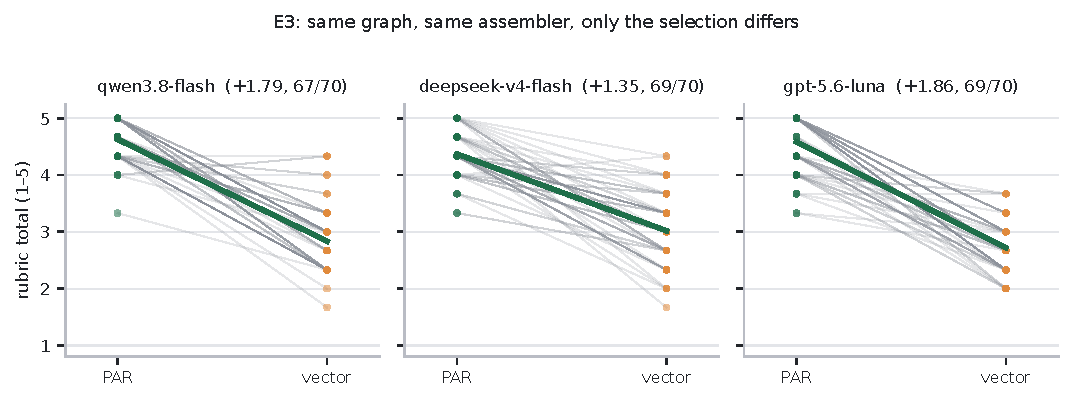
\includegraphics[width=\linewidth]{fig2_e3_paired.pdf}
  \caption{E3 per-query pairing ($n=70$). Thin lines are queries, the thick line is the mean;
  the three panels are the three judges. Same graph, same assembler, only the selection differs.}
  \label{fig:e3}
\end{figure}

Figure~\ref{fig:e3} shows the same result query by query: almost every line slopes upward under
every judge.

\subsection{Mechanism Ablation (E4): Scores Tie, Products Diverge}
\label{sec:e4}

Starting from the best E3 combination (PAR plus narrative assembly), we switch off one mechanism
at a time, in two batches (Table~\ref{tab:e4batches}).

\begin{table}[t]
  \centering
  \small
  \begin{tabular}{@{}llp{0.55\linewidth}@{}}
    \toprule
    Batch & Conditions & How the mechanism is removed \\
    \midrule
    Purpose & full / no\_purpose / random\_purpose & the whole purpose channel is disabled
      (no inference, no purpose seeds, no filtering, no purpose term in the score); random
      purposes are drawn from real node text \\
    Structure & full / no\_jump\_axis / no\_peak\_band & jump weights set to 1.0; band width set to
      10 (equivalent to no filtering) with equal-size truncation \\
    \bottomrule
  \end{tabular}
  \caption{E4: ablation batches.}\label{tab:e4batches}
\end{table}

At the score level, pairwise differences among the five conditions are only 0.02--0.15, and the
sign is inconsistent across judges (full $-$ no\_purpose: qwen $+0.06$, deepseek $+0.11$,
gpt $-0.15$).

The filter branch of \emph{full} must be stated explicitly: with the default $\tau=0.30$ on the
163-node graph, no candidate is removed---the mean cosine between the 70 injected purposes and
all nodes is 0.500, and the minimum is still above 0.30. The difference between \emph{full} and
\emph{no\_purpose} therefore comes from purpose seeding and weighting, not filtering. E4 answers
whether an abstract purpose vector is a useful seeding/weighting signal; it cannot answer whether
purpose filtering helps (see Sections~\ref{sec:e10} and~\ref{sec:e11}).

At the product level (70 queries; only the node sets of full and no\_purpose are rebuilt), the
picture is different (Table~\ref{tab:e4product}).

\begin{table}[t]
  \centering
  \small
  \begin{tabular}{@{}lcc@{}}
    \toprule
    Metric & full & no\_purpose \\
    \midrule
    gold-facet recall & 0.857 & \textbf{0.894} \\
    mean nodes & \textbf{33.1} & 22.3 \\
    node-set Jaccard between the two & \multicolumn{2}{c}{0.310} \\
    queries with more hits & 8 & \textbf{13} (49 ties) \\
    \bottomrule
  \end{tabular}
  \caption{E4: the mechanism changes the product, but not in a consistently better direction.}
  \label{tab:e4product}
\end{table}

Three conclusions follow. First, the mechanism does change the product substantially (Jaccard
0.31), so a tied score does not mean an inactive mechanism; it means the three-dimensional rubric
is insensitive to this kind of difference. Here the mechanism is purpose seeding/weighting, not
filtering. Second, the direction is often wrong: removing the purpose channel gives \emph{higher}
recall, and full emits 50\% more nodes without a higher hit rate; these extra nodes are brought in
by purpose seeds/weights and behave as noise under the current representation. Third, effectiveness
depends on the query type (Table~\ref{tab:e4types}).

\begin{table}[t]
  \centering
  \small
  \begin{tabular}{@{}p{0.24\linewidth}p{0.22\linewidth}p{0.44\linewidth}@{}}
    \toprule
    Query type & Behaviour & Example (gold recall) \\
    \midrule
    single topic, clear intent & full clearly better & q21 ``plan and split my tasks''
      0.56 vs 0.44; q09 ``lost $\rightarrow$ programming'' 1.00 vs 0.80 \\
    cross-scenario, mixed & full clearly worse & q11 ``boring project, want a two-day weekend
      team'' 0.33 vs \textbf{1.00}; q52 0.33 vs \textbf{1.00}; q20 0.50 vs \textbf{1.00} \\
    \bottomrule
  \end{tabular}
  \caption{E4: the effect flips with query type.}\label{tab:e4types}
\end{table}

The mechanism is visible in the representation. Injected purpose phrases are abstractions
(``prepare to change teams''), which land closer to planning and advice nodes than to concrete
facts (``worked until eleven'', ``wants a team with two-day weekends''). On single-topic queries
the two node groups overlap, so the abstraction still works; on cross-scenario queries it pulls
retrieval into planning branches and squeezes out the facts. The same trade-off explains the tied
total: full is rewarded for richness (33 vs 22 nodes) and penalised for user modeling (lower
recall), and the two cancel.

\subsection{Intent Conditioning (E5)}
\label{sec:e5}

The design changes the \emph{purpose}, not the text. Each scenario has one sentence that does not
name an intent, plus three purpose sets (vent / plan / recommend) and a gold facet per intent.
The three arms are \texttt{par} (purpose seeds, filtering, and weighting), \texttt{vector\_purpose}
(text and purposes concatenated before embedding), and \texttt{vector\_text} (text only, an
internal lower bound). Table~\ref{tab:e5} reports the result.

\begin{table}[t]
  \centering
  \small
  \begin{tabular}{@{}lccc@{}}
    \toprule
    Metric & par & vector\_purpose & vector\_text \\
    \midrule
    Jaccard across intents (lower = more differentiated) & 0.343 & 0.319 & \textbf{0.652} \\
    gold-facet recall & 0.594 & \textbf{0.697} & 0.362 \\
    \bottomrule
  \end{tabular}
  \caption{E5: three arms on 30 items (10 scenarios $\times$ 3 intents).}\label{tab:e5}
\end{table}

One conclusion is clean: plain text is almost blind to purpose (0.652 vs 0.32--0.34), which
supports the premise that purpose must enter retrieval explicitly. But par is on par with the
simplest concatenation, and its recall is lower: the purpose handling of PAR does not beat naive
text concatenation.

A node-type breakdown (Table~\ref{tab:e5types}) shows why. The total-variation distance (TVD)
between intents is only 0.042--0.066; when the user vents, emotion nodes account for 10.6\%, which
is indistinguishable from planning (9.4\%) and recommending (10.1\%). All three intents drift to
action nodes.

\begin{table}[t]
  \centering
  \small
  \begin{tabular}{@{}lcccc@{}}
    \toprule
    Intent & status & action & emotion & thing \\
    \midrule
    vent & 16.3\% & 45.8\% & \textbf{10.6\%} & 23.9\% \\
    plan & 12.1\% & 49.1\% & 9.4\% & 27.2\% \\
    recommend & 14.1\% & 45.4\% & 10.1\% & 28.2\% \\
    \bottomrule
  \end{tabular}
  \caption{E5: node-type mix of the retrieved sets.}\label{tab:e5types}
\end{table}

Gold recall by intent is vent 0.642/0.675, plan 0.617/0.825, and recommend 0.525/0.592 for
par/vector\_purpose; the second arm wins on all three. The Jaccard gap in E5 therefore comes from
retrieving different nodes, but the difference is a permutation \emph{within} the same type, not
a move toward the type the intent needs.

\subsection{Failure Taxonomy (E9)}
\label{sec:e9}

Seventy-six Ariadne products were coded with LLM assistance (not double human annotation; used
only for distribution estimates and case selection). Table~\ref{tab:e9} reports the distribution.

\begin{table}[t]
  \centering
  \small
  \begin{tabular}{@{}lcc@{}}
    \toprule
    Failure type & Hits & Share \\
    \midrule
    cross-domain context & 70 & \textbf{92.1\%} \\
    over-story (inferred additions) & 43 & 56.6\% \\
    intent miss & 19 & 25.0\% \\
    redundancy & 11 & 14.5\% \\
    missing explicit constraint & 3 & 3.9\% \\
    purpose error (overall drift) & 2 & \textbf{2.6\%} \\
    \bottomrule
  \end{tabular}
  \caption{E9: failure taxonomy over 76 products.}\label{tab:e9}
\end{table}

The dominant failure is not ``searching in the wrong direction'' but ``bringing too much along''
(92.1\% vs 2.6\%). This is consistent with the E5 product composition and with the cross-subject
contamination in E10: the weakness is precision and focus, not recall direction.

The 92.1\% figure is specific to the \emph{strict service} standard. Re-judging the same probe
under a user-modeling standard (any true fact about the same user counts as 0 even if irrelevant
to the current request) gives 96.3\% under the strict standard but 0\% under the user-modeling
standard (27 items). The number is therefore a consequence of the chosen standard, not an absolute
rate of narrative drift. The permissive standard is close to tautological, however, so it cannot
be used to argue that the narratives are useful. The figure must be cited with the strict-standard
qualifier.

\subsection{Output Stability (E7)}
\label{sec:stability}

With purposes injected and inference randomness removed, 70 queries were rerun three times
(Table~\ref{tab:e7}).

\begin{table}[t]
  \centering
  \small
  \begin{tabular}{@{}lcccc@{}}
    \toprule
    Arm & node-set Jaccard & $p_{05}$ & identical in 3/3 & node-count range \\
    \midrule
    par & \textbf{0.764} & 0.425 & 8/70 & 7.5 \\
    vector\_purpose & 0.871 & 0.610 & 8/70 & 7.5 \\
    \bottomrule
  \end{tabular}
  \caption{E7: rerun stability (three runs per query).}\label{tab:e7}
\end{table}

A single run carries considerable jitter, caused by tiny non-determinism in the remote embedding
service (the same text can swap rank between two calls). This is why every comparison in the
paper is stated only when the difference is at least 0.2.

\subsection{Data Separability and Thresholds (E10)}
\label{sec:e10}

Testing the purpose filter requires a graph whose scenarios are actually separable. We add two
unrelated subjects to the original 163 nodes (90 memories of a 45-year-old secondary-school
teacher, 90 of a 28-year-old cross-border e-commerce operator), giving L / M / H graphs, and use
ROC AUC (same subject and scenario vs.\ the rest) as the common yardstick
(Table~\ref{tab:e10auc}).

\begin{table}[t]
  \centering
  \small
  \begin{tabular}{@{}lcccccc@{}}
    \toprule
    Graph & Nodes & Within & Across & Gap & AUC & Best margin \\
    \midrule
    L & 163 & 0.585 & 0.518 & 0.068 & 0.717 & 0.334 \\
    M & 253 & 0.576 & 0.504 & 0.072 & 0.744 & 0.374 \\
    H & 343 & 0.569 & 0.493 & 0.077 & 0.767 & 0.403 \\
    \bottomrule
  \end{tabular}
  \caption{E10: cosine separability across graph sizes.}\label{tab:e10auc}
\end{table}

Node-level bootstrap 95\% CIs (2,000 resamples) are L $[0.689,0.767]$, M $[0.724,0.786]$, and
H $[0.753,0.805]$; the three intervals overlap, so the pattern cannot be read as ``AUC rises with
scale''. Adding two unrelated people does not significantly improve separability; under
bge-large-zh-v1.5 only L--H is marginally separated ($[0.673,0.750]$ vs.\ $[0.752,0.806]$). On
bge-m3 the cosine between two different subjects is still 0.493. Because AUC is a ranking metric,
no monotone threshold transform (absolute, relative, or quantile) can break through it.
Figure~\ref{fig:e10} summarizes both panels.

The partial AUC (FPR $\le0.10$, normalised by the random baseline) is \textbf{3.74 / 5.00 / 5.55}
for m3 and \textbf{4.22 / 5.60 / 6.21} for zh-1.5: the high-score region is more separable than
the global AUC. Yet TPR at FPR$=10\%$ is only 0.33 / 0.41 / 0.43 (m3) and 0.36 / 0.44 / 0.46
(zh-1.5), so a local operating point exists at the cost of losing more than half of the positives.

\begin{figure}[t]
  \centering
  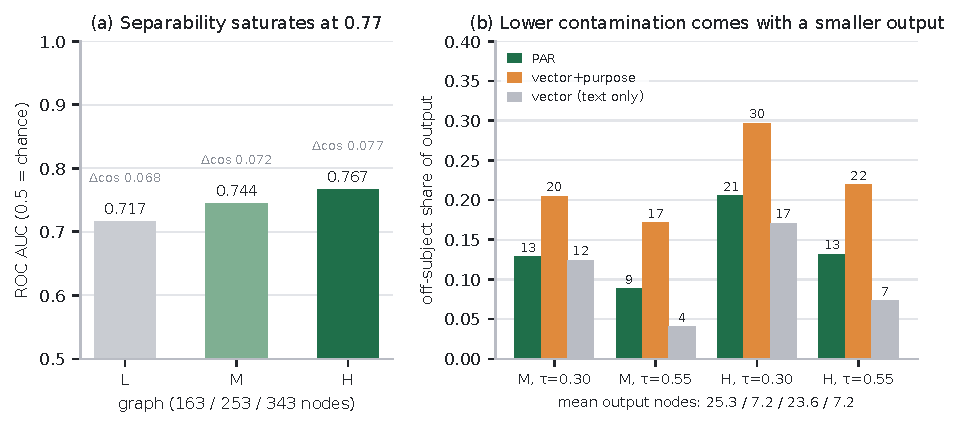
\includegraphics[width=\linewidth]{fig3_e10_tradeoff.pdf}
  \caption{(a) Same-subject vs.\ cross-subject separability (ROC AUC, 0.5 = chance); the label
  above each bar is the difference between the two cosine means. (b) Cross-subject share of the
  output as a function of threshold and graph size; the label under the axis is the mean output
  size. The three arms are PAR, text-plus-purpose concatenation, and text only.}
  \label{fig:e10}
\end{figure}

Table~\ref{tab:e10filler} reports the filler effect, i.e.\ the share of the output that belongs
to another subject.

\begin{table}[t]
  \centering
  \small
  \begin{tabular}{@{}llcccc@{}}
    \toprule
    Graph & $\tau$ & par & vector\_purpose & vp + same $\tau$ & vector\_text \\
    \midrule
    M & 0.30 & \textbf{12.9\%} & 20.5\% & 20.3\% & 12.4\% \\
    M & 0.55 & \textbf{8.8\%} & 17.1\% & 17.1\% & 4.0\% \\
    H & 0.30 & \textbf{20.6\%} & 29.7\% & 29.6\% & 17.1\% \\
    H & 0.55 & \textbf{13.2\%} & 21.9\% & 21.9\% & 7.3\% \\
    \bottomrule
  \end{tabular}
  \caption{E10: cross-subject share under different thresholds.}\label{tab:e10filler}
\end{table}

PAR is 7--9 points lower than the unthresholded vector arm (winning 13--20 of 30 queries), but
this is \emph{not} the contribution of the threshold gate: the vector arm with the same $\tau$ is
within 0.2 pp of the unthresholded arm, and on the 163-node graph $\tau=0.30$ removes no node at
all. The 7--9 pp gap comes from PAR's selection mechanism (graph expansion, purpose seeds, and
weighting). The filter starts to bite only at 0.45--0.55: output drops from about 25 to 7--8 nodes
and contamination falls, but this is zero-sum rather than a free precision gain. Text-only
retrieval is always the cleanest (4.0\% / 7.3\%).

We tried three repairs (a seed cosine floor, a relative threshold $\mu+k\sigma$, and more
concrete purposes). In the full run, the relative threshold trades roughly 1:1 recall for
contamination, the seed floor does nothing, and more concrete purposes \emph{increase}
contamination by 1.6--3.2 pp. In the range where the filter actually works (0.45--0.55), tuning
cannot improve precision and recall together, for the reason given in Section~\ref{sec:zerosum}.

Cost (formerly E8) is not measured separately: it affects only the cost paragraph, not any
conclusion, and gateway queueing makes latency irreproducible. Qualitatively, PAR adds one graph
expansion; assembly is identical to the vector arms.

\subsection{Structured Purpose (E11)}
\label{sec:e11}

Section~\ref{sec:e5} shows that the purpose channel is not working. Section~\ref{sec:discussion}
locates the cause in the representation: three purpose phrases describe the same topic and become
nearly the same vector, so retrieval can tell ``similar'' but not ``which kind of content.''
Here we run a minimal test: change only how the purpose is written, and leave the retrieval
mechanism untouched.

The purpose is split into three requirements: the target content type (state, feeling, action,
object, person, cause), the expected relation type (cause, order, similarity, attribute), and the
episode the user is talking about, anchored to the original utterance. The three are combined
multiplicatively, so a candidate must first belong to the episode and only then be ranked by type
(Section~4.3). The first version was additive; ``right type, wrong episode'' memories were then
pulled up, and the average hit rate on one scenario fell from 0.58 to 0.23. The multiplicative
gate restores it to 0.60. Table~\ref{tab:e11} reports the comparison, and
Table~\ref{tab:e11example} walks through one scenario.

\begin{table}[t]
  \centering
  \small
  \begin{tabular}{@{}lcccc@{}}
    \toprule
    Threshold & Type divergence (per scenario) & Type divergence (pooled)
              & Gold-facet recall & Mean output size \\
    \midrule
    0.30 & 0.240 $\rightarrow$ 0.256 & 0.137 $\rightarrow$ 0.166 & 0.277 $\rightarrow$ 0.330 & 9.5 $\rightarrow$ 10.0 \\
    0.40 & 0.246 $\rightarrow$ \textbf{0.422} & 0.119 $\rightarrow$ \textbf{0.372} & 0.289 $\rightarrow$ \textbf{0.512} & 9.5 $\rightarrow$ 9.0 \\
    0.45 & 0.272 $\rightarrow$ \textbf{0.524} & 0.090 $\rightarrow$ \textbf{0.473} & 0.301 $\rightarrow$ \textbf{0.529} & 9.5 $\rightarrow$ 7.6 \\
    0.50 & 0.245 $\rightarrow$ \textbf{0.486} & 0.094 $\rightarrow$ \textbf{0.440} & 0.456 $\rightarrow$ 0.460 & 8.7 $\rightarrow$ 6.1 \\
    \bottomrule
  \end{tabular}
  \caption{E11: flat purpose versus structured purpose (30 items, same budget of at most 10
  nodes; each cell is flat $\rightarrow$ structured).}\label{tab:e11}
\end{table}

At threshold 0.30 nothing changes. The reason is not that the representation fails, but that the
multiplicative gate lowers the whole score scale: the old threshold blocks nothing (0.91 of
candidates pass per round). At 0.45 the filter starts to work (0.30 pass). The threshold must be
recalibrated together with the representation, which is the general problem of
Section~\ref{sec:zerosum}.

Frame and filter must be separated. With the same budget of at most 10 nodes, a same-batch rerun
of frame-only ($\tau=0$) already gives TVD 0.27--0.34. The natural TVD at 0.45 (0.52) is mainly
due to output shrinking from 10 to 7.5--7.9 nodes; at equal node count the TVD is only 0.29--0.36. The
independent contribution of filtering is higher gold-facet recall (+24--29 pp) and lower
cross-subject contamination ($-4$ to $-7$ pp) at equal size, at the cost of removing 4--6\% of
gold. The TVD gain in E11 is therefore attributable to frame plus output budget, not to cosine
filtering itself.

\begin{table}[t]
  \centering
  \small
  \begin{tabular}{@{}llc@{}}
    \toprule
    Purpose & Dominant content retrieved & Hits \\
    \midrule
    vent & worked until eleven, irritated by the new request, exhausted, the cause of overtime
         & 4/4 \\
    plan & next week, the schedule list, the Wednesday review, the task-splitting script
         & 4/5 \\
    recommend & advice on study anxiety, a load-testing tool (from another episode) & 0/3 \\
    \bottomrule
  \end{tabular}
  \caption{E11: one scenario (``I have been really tired this week'') at threshold 0.45.}
  \label{tab:e11example}
\end{table}

\paragraph{Boundaries.}
First, the three requirements currently come from a hand-written mapping (``vent'' implies
feeling first), and four of five free-form purposes are not recognised (``I want to be heard,''
``help me persuade my mother''); unrecognised purposes fall back to the old method. The
representation is validated; obtaining it automatically is not. Second, the threshold must be
recalibrated. Third, ``recommend'' remains weak: in the graph, ``the assistant compared several
options'' and ``the assistant said something'' are the same node type, so type alone cannot
separate them. Fourth, evaluation is at the retrieval level only (30 items, one graph, one
embedding model, no judge). Fifth, the gain presupposes that the content an intent needs is
separable by type; if it is not, the type distribution separates while the hit rate does not.


\section{Discussion}
\label{sec:discussion}

\subsection{What Each Layer of Evidence Answers}
\label{sec:layers}

The evidence comes in three layers, and the boundaries must be kept apart
(Table~\ref{tab:layers}).

\begin{table}[t]
  \centering
  \small
  \begin{tabular}{@{}llp{0.3\linewidth}p{0.3\linewidth}@{}}
    \toprule
    Layer & Experiment & Answers & Cannot answer \\
    \midrule
    System & E1 & whether the full pipeline yields more useful context & whether PAR is responsible \\
    Mechanism & E3 & how large the difference is under the same graph and assembler &
      how much each sub-mechanism contributes \\
    Sub-mechanism & E4 / E5 / E10 / E11 & whether the purpose channel works as intended &
      how much end-to-end quality a better purpose representation would add \\
    \bottomrule
  \end{tabular}
  \caption{Three evidence layers.}\label{tab:layers}
\end{table}

E1 and E3 together support the claim that associative selection on the graph beats vector
top-$k$; the C$-$D contrast in E3 has $r\approx1.00$ under all three judges and is the most
stable result here. The studies from E4 onward show that, with the purpose representation used
in the main pipeline, the sub-mechanism layer does not yet produce a gain; what changes when the
purpose is written differently is reported in Section~\ref{sec:e11}.

\subsection{The Purpose Representation Is the Bottleneck}
\label{sec:bottleneck}

This is the main negative result, and it rests on five independent lines of evidence:

\begin{enumerate}
  \item \textbf{E4, product level.} The node sets of full and no\_purpose have a Jaccard of only
        0.31, so the mechanism is active; yet no\_purpose has higher gold recall (0.894 vs 0.857)
        and wins more queries (13 vs 8).
  \item \textbf{E4, query type.} Full is better on single-topic queries and clearly worse on
        cross-scenario queries (0.33 vs 1.00).
  \item \textbf{E5, intent level.} The TVD between intents is only 0.04--0.07; under venting,
        emotion nodes make up 10.6\%, no different from planning or recommending.
  \item \textbf{E10, interference level.} The main cause of cross-subject contamination is not
        the threshold scale but the fact that queries and ``summary sentences about another
        subject'' are already close in embedding space (AUC ceiling 0.767).
  \item \textbf{E10/E11, threshold level.} The default $\tau=0.30$ removes no node on the main
        graph (the mean purpose--node cosine is 0.500 and the minimum is still above 0.30), so the
        negative result in E4/E5 concerns purpose seeds and weighting, not filtering. The filter
        starts to work at 0.45 and then trades output size for precision. An abstract
        representation therefore not only steers in the wrong direction but also leaves the filter
        branch nominally present and functionally inactive.
\end{enumerate}

All five point to one mechanism: \emph{when a purpose is represented as a pooled vector of
abstract phrases, it lands in the ``summary / plan / advice'' region of the semantic space and
cannot steer retrieval toward the concrete facet the intent needs.} On single-topic queries the
two node groups coincide, hiding the problem; on cross-scenario queries the shift becomes
visible.

The resulting order is: \emph{fix the representation first (frame / three requirements), then
calibrate the threshold}. Tuning $\tau$ alone cannot create discrimination.

Two testable directions follow. The first is \emph{structuring the purpose} into the content
type, the relation type, and the episode, instead of one abstract phrase vector.
Section~\ref{sec:e11} implements it: with the three requirements supplied, the pooled type
divergence rises from 0.09 to 0.47 and gold-facet recall from 0.30 to 0.53, but the requirements
themselves are still hand-written. The remaining problem is obtaining them automatically
(Section~\ref{sec:future}). The second is \emph{grounding the purpose in facts} (``the user said
they were tired, worked until eleven, wants a two-day weekend'') so that the vector lands near
fact nodes. This direction is not implemented here.

\subsection{The Zero-Sum Nature of Threshold Tuning}
\label{sec:zerosum}

E10 shows that, on the same graph, same-subject and cross-subject cosine distributions overlap
heavily (AUC 0.717--0.767). Under that condition, any \emph{monotone} threshold, whether
absolute $\tau$ or relative $\mu+k\sigma$, can only move along the same ROC curve: lowering
contamination costs an equal amount of recall. Empirically, in the 0.45--0.55 range, the relative
threshold lowers contamination by 7.8 pp while losing 9.8 pp of recall, roughly 1:1.

Two regimes must be distinguished. $\tau=0.30$ is not an operating point on the main graph (it
removes no node), so ``zero-sum'' does not even apply there. $\tau\approx0.55$ is a local
operating point: contamination falls while output shrinks from about 25 to 7 nodes, and zero-sum
holds in that range. A quantile threshold $\tau=Q_{1-p}(\cos)$ replaces the absolute value with a
retention ratio. At the same $p$, contamination varies across graphs by 3.5--3.9 pp (m3 and
zh-1.5), so $p$ is portable for contamination; output size and gold recall at the same $p$ scale
with graph size, so the budget is not portable. The partial AUC of $3.7$--$6.2\times$ chance
likewise shows that the high-score region is more separable, but TPR at FPR$=10\%$ is only
0.33--0.46, so the local operating point still loses positives.

Two corollaries follow. First, ``tuning the threshold to the right value'' is not a solvable
engineering problem unless the space is changed first, either by a different representation or
by different data. Second, the value of a relative threshold ($\mu+k\sigma$) is
\emph{portability across embedding models}: the meaning of an absolute $\tau$ drifts with the
model (the same unrelated text scores 0.405 on bge-m3 and 0.269 on bge-large-zh), but the
relative form does not. It is not a way to improve effectiveness.

\subsection{Relation to Retrieval Metrics}
\label{sec:metrics}

We do not deny the value of P@K and R@all for question-answering retrieval. Here they serve only
as mechanism diagnostics: whether the jump axis expands, whether purpose filtering blocks
semantic neighbours, and whether the peak band retains multi-hop candidates. Three process
metrics replace ranking: node-set Jaccard for differentiation, gold-facet recall for direction,
and cross-subject or cross-scenario contamination for precision.

\subsection{When PAR Does Not Apply}
\label{sec:notapply}

\begin{itemize}
  \item question answering that requires exact answer localisation: a set is the wrong shape;
  \item noisy memory graphs with unreliable type labels: the jump axis amplifies the errors;
  \item purposes available only as abstract phrases: this introduces a systematic shift
        (Section~\ref{sec:bottleneck});
  \item settings that require interpretable threshold semantics: absolute thresholds do not
        transfer across models (Section~\ref{sec:zerosum}).
\end{itemize}

\subsection{Future Work}
\label{sec:future}

We leave three pieces of work to later contributors, because each needs controlled large-scale
data that this study does not have.

\paragraph{(i) Calibrating and learning the jump-axis weights.}
The $6\times8$ matrix is a hand-specified prior. We only ran coarse ablations (all zeros, all
ones); there is no sensitivity analysis and no data-driven fit, so we cannot say how far the
current weights are from optimal. A useful path is to perturb each of the 48 cells by $\pm50\%$,
identify the high-sensitivity cells (CAUSAL and SCENARIO are likely), then relax the discrete
weights into continuous parameters and optimise them with weak supervision from gold-facet hits.
Acceptance: on a controlled graph, the learned weights reproduce the behaviour ``keep only
relevant branches when the seed fans out'', and recall on real graphs does not fall below the
hand-set prior.

\paragraph{(ii) Parameters for graphs of different size and type.}
$\tau$, $\delta$, and $k$ are fixed at 0.30, 0.10, and 5. Section~\ref{sec:e10} shows that they
are tightly coupled to the separability of the data, but we give no portable calibration rule.
Order matters: when the purpose vector has a cosine of about 0.50 to every node, no $\tau$ can
create discrimination; calibration must follow, not replace, the representation fix. A
structured grid (100 / 500 / 2000 nodes $\times$ out-degree 2 / 5 / 10 $\times$ AUC 0.7 / 0.8 /
0.9) would allow fitting $\tau=q_p(\cos)-c\cdot\mathrm{IQR}(\cos)$ and
$\delta=\lambda(\mu_{\text{peak}}-\mu_{\text{tail}})$ and testing them on held-out graphs.
Acceptance: within 5\% of the grid-search optimum on the held-out graphs.

\paragraph{(iii) Turning free-form purposes into the three requirements.}
Section~\ref{sec:e11} validates the representation but the three requirements are produced by a
hand-written mapping; four of five free-form purposes are not recognised. Nodes carry a
\texttt{timestamp} field written from the batch time, but the retrieval path does not use a time
window or time filter; there is also no structured subject field, so ``time window'' and ``whose
episode'' are only approximated. A workable path is to compile the frame with a model, using a
small set of human annotations as seeds and calibrating the compilation against human labels
rather than only against downstream metrics; the retrieval path would need to consume the
existing time field, and the schema a structured subject field.
Acceptance: at least 80\% of free-form purposes yield a non-empty frame (currently 1 in 5), the
E11 protocol still gives $\mathrm{TVD}>0.2$ and recall no worse than the hand-written frame, and
the result holds for intents outside vent / plan / recommend.

\section{Limitations}
\label{sec:limitations}

\begin{enumerate}
  \item \textbf{Scale and ecological validity.} 163 nodes, 237 edges, 76 queries, manually
        constructed. The conclusions are limited to the emotional-companion setting. The mechanism
        ordering is stable under an auto-built graph, structural perturbations, and an embedding
        swap (C$-$D 1.16--1.63, $r\ge0.96$), but this is still one scenario and one graph family.
  \item \textbf{Insufficient data separability, and an inactive default threshold.}
        Same-scenario and cross-scenario cosine distributions overlap heavily (ROC AUC
        0.717--0.767; the three confidence intervals overlap). The default $\tau=0.30$ removes no
        node on this graph and is therefore equivalent to no filtering. A local operating point
        appears only near $\tau\approx0.55$, where contamination falls at the cost of output size
        (zero-sum). A quantile threshold can align contamination across graphs (range below 5 pp)
        but not the output budget. We therefore cannot validate the net benefit of purpose
        filtering with an absolute threshold; the result is only ``does not hold under the current
        representation and default configuration''. In E11 the threshold does start to work, but
        it is a recalibrated threshold and does not vindicate the old value of 0.30.
  \item \textbf{Noticeable jitter in a single run.} Rerunning the same query three times gives a
        node-set Jaccard of 0.764 (8/70 identical), caused by tiny non-determinism in the remote
        embedding service. Differences below 0.2 are therefore not treated as conclusions.
  \item \textbf{E1 and E3 products were not generated at the same time.} Ariadne was rerun with
        the current pipeline, whereas Graphiti and Mem0 outputs come from an archive. We
        recalibrated the judge on archived blocks, but differences in extraction versions cannot
        be fully excluded; the E1 margin is directional evidence. The E3 main table is also the
        archived bandfix batch (C$-$D 1.296); a same-batch rerun gives 1.633, a difference of 0.34
        that exceeds the 0.2 noise band, so robustness checks use only the same-batch baseline.
  \item \textbf{LLM judges.} $\alpha=0.657$ (E1) and 0.774 (E3) are moderate to good, not human
        agreement, and reliability varies with effect size.
  \item \textbf{E9 is LLM-assisted coding.} The labels depend on a model comparing ``available
        facts''; they are suitable for distribution estimates and case selection, not for precise
        proportions.
  \item \textbf{No human user study.} We evaluate whether the context supports user modeling, not
        whether users feel understood.
  \item \textbf{No fixed golden set, a double-edged choice.} It avoids treating one intent as the
        only correct one, but it also reduces comparability with other benchmarks.
  \item \textbf{The peak band deviates from its design intent.} The design is ``stop at the first
        peak''; the current implementation resets its timer when the score rises again and thus
        goes deeper on multi-peak chains. A controlled experiment shows that first-peak stopping
        removes 19\% of the output for 0.8 pp of recall, but the main numbers here use the current
        implementation ($\text{patience}=2$).
  \item \textbf{The E11 demonstration has clear boundaries.} The three requirements are given by
        a hand-written mapping (four of five free-form purposes are not recognised), the
        threshold is scanned rather than derived, evaluation is retrieval-level only (30 items,
        one graph, one embedding model, no judge), and the conclusion assumes that the content an
        intent needs is separable by type. Moreover, part of the natural TVD gain comes from a
        smaller output; at equal node count the increment is small (Section~\ref{sec:e11}). It
        demonstrates that the representation works, not that the purpose channel already yields
        end-to-end gains.
  \item \textbf{Ethics.} Dialogue data are synthetic or de-identified and contain no real private
        information. Judges may carry language and cultural bias; anonymisation and per-query
        shuffling only partially control for it.
\end{enumerate}

\section{Conclusion}
\label{sec:conclusion}

We recast dialogue-memory retrieval from ``find relevant documents'' to ``model the current
user'', and propose PAR: direction-aware typed expansion, purpose regression, and a
peak-tolerance output band, evaluated with an LLM-judged protocol that does not assume a fixed
golden set.

On 76 statement-style queries in an emotional-companion scenario:

\begin{itemize}
  \item \textbf{System level:} the full system ranks first under all three judges, with
        differences of $+0.69$ to $+1.80$ over Graphiti and Mem0 ($p\le10^{-8}$).
  \item \textbf{Mechanism level:} on the same graph with the same assembler, changing only the
        selection mechanism improves scores by $+1.35$ to $+1.86$ over vector top-$k$, with
        rank-biserial $r\approx1.00$ under all judges.
  \item \textbf{Sub-mechanism level:} the purpose channel changes the retrieved product
        substantially (node-set Jaccard 0.31), but under the pooled-phrase representation the
        change is right about half the time and does not translate into end-to-end or gold-facet
        gains.
\end{itemize}

The claim is therefore conditional. Associative selection on the graph (jump axis, peak band,
set output) is a stable source of gain in this setting. The purpose-driven layer has not yet
converted into a gain in its current form. Two qualifications matter. First, the default
$\tau=0.30$ filter is inactive on the main graph, so the negative result concerns the abstract
purpose vector as a seeding/weighting signal, not purpose filtering as such. Second, the filter
enters a zero-sum regime at 0.45--0.55, where it trades output size for precision.
Section~\ref{sec:e11} shows that rewriting the purpose
as content type, relation type, and episode raises the type divergence from 0.09 to 0.47 and
recall from 0.30 to 0.53, but this depends on hand-supplied requirements; obtaining them from
arbitrary phrasing is what remains.

PAR is not a stronger RAG but a solution to a different problem. Its value is to move the object
of evaluation from a ranked list to a user-modeling context, to give this still standard-less
area a reproducible starting point, and to state clearly where the current ceiling is.

\appendix

\section{Old Retrieval Metrics (Diagnostics Only)}
\label{app:oldmetrics}

The numbers below come from earlier 47/83/216-node synthetic data and an A/B/C comparison. They
are not used in the main text; they only show whether the mechanism behaves as intended.
Table~\ref{tab:oldmetrics} lists them.

\begin{table}[ht]
  \centering
  \small
  \begin{tabular}{@{}lccc@{}}
    \toprule
    Condition & P@5 & R@all & Note \\
    \midrule
    A (vector only) & 0.267 & 0.159 & fixed 5 \\
    B (undirected graph mix) & 0.267 & 0.159 & $\alpha=0.5$ fixed \\
    C (jump axis only) & --- & 0.267 & P@5 not reported separately \\
    PAR (full) & 0.160 & \textbf{0.538} & 6--27 nodes \\
    \bottomrule
  \end{tabular}
  \caption{Historical retrieval metrics on 216 nodes.}\label{tab:oldmetrics}
\end{table}

\paragraph{Correction.}
C's R@all is 0.267; an earlier table mistook it for P@5 and copied A's 0.159 into C's R@all.
C's P@5 was never reported separately. A and B share the same P@5/R@all because they use the same
fixed $\alpha=0.5$ configuration; this is not a tuned version of B.
Table~\ref{tab:oldablation} summarizes the early ablations.

\begin{table}[ht]
  \centering
  \footnotesize
  \setlength{\tabcolsep}{4pt}
  \begin{tabular}{@{}lp{0.22\linewidth}p{0.42\linewidth}@{}}
    \toprule
    Ablation & Observation & Interpretation \\
    \midrule
    A2: jump axis all zeros & R@all falls back to A (0.159), only 6 unique hits &
      the jump axis is the source of graph signal; A2 has no net recall gain \\
    A1: purpose filter removed & on the early small graph, many semantic neighbours entered and
      user-modeling scores dropped & \textbf{not reproduced} on 163 nodes: scores tie (0.02--0.15,
      unstable sign) and gold recall is higher without it (0.894 vs 0.857) \\
    A3/A4/A8: weight variants & output size changes, score direction unstable &
      the weight matrix is a hand-set prior and needs a sensitivity analysis \\
    A5: random purpose & output decouples from the real purpose & the purpose vector is not
      decorative \\
    fixed hops: no peak band & long paths truncated, or many irrelevant nodes kept &
      the band keeps multi-hop candidates near the peak \\
    \bottomrule
  \end{tabular}
  \caption{Early ablation summary (47/83/216-node data).}\label{tab:oldablation}
\end{table}

\paragraph{Why this is in the appendix.}
PAR does not produce a ranked list, so P@5 is undefined; R@all depends on a fixed expected set,
which does not hold in dialogue; and output sizes are not comparable, so R@all rewards returning
more. These numbers are mechanism diagnostics, not a system ranking.

\section{Evaluation Materials}
\label{app:materials}

The artifact contains the judge rubric (three dimensions, 1--5), the side-by-side prompt, the
anonymisation and shuffle rules, the category distribution of the 76 queries, failure cases with
short excerpts, and the data and model versions with dates.

\section{Reproducibility and Version}
\label{app:repro}

\begin{itemize}
  \item Data: 163 nodes / 237 edges, 26 dialogue batches, 76 queries; an intent set of 10
        scenarios $\times$ 3 intents (E5; E11 reuses the same 30 items); and L / M / H graphs
        (163 / 253 / 343 nodes, E10).
  \item Systems: Ariadne, Mem0 (Chinese patch), Graphiti (self-hosted with Neo4j).
  \item Judges: qwen3.8-flash, deepseek-v4-flash, gpt-5.6-luna. gemini-3.7-flash was removed
        from the main table because of system-name confusion and gateway timeouts; its outputs
        are kept for reference only.
  \item Scoring: temperature 0, structured output, side-by-side presentation, per-query
        anonymised shuffling; stability is measured separately by E7 (three reruns).
  \item Code, data, and prompts are released with the preprint artifact.
  \item Version: v0.5.1, 2026-11-19. Relative to v0.5 this revision only adds the archived
        DOIs; no result changes. v0.5 added bootstrap confidence intervals (E14),
        pAUC and quantile thresholds (E13), graph-source and structural-perturbation checks
        (E12a/E12b), and an embedding swap (E15c); it also corrects the attribution of the
        0.30 filter, the 7--9 pp contamination gap, and the E9 92.1\% figure.
        Later versions will add a real-user study, threshold validation under a stronger
        representation, and larger judge replication.
\end{itemize}

\section{Graph Construction and Maintenance (Summary)}
\label{app:dba}

This paper treats the memory graph as an input. The main experiments use a manually built graph;
the automatic graph in \S\ref{sec:e3} is produced by a DBA pipeline. The full description is in a
companion technical report included with the artifact; we only summarise the
minimum needed for reproduction.

\begin{itemize}
  \item Maintenance runs asynchronously after each dialogue batch. The LLM receives the raw
        dialogue, semantically related memories ($k=15$), and the structural neighbourhood
        ($k=5$, truncated to 20), and emits create / update / fix\_type / deprecate /
        create\_edge / delete operations.
  \item The six node types and eight relation types are those in \S\ref{sec:graph}; deduplication
        uses cosine threshold 0.85 in the prototype and 0.92 in production; the orphan counter is
        3 in the prototype and disabled in production; there is no time decay.
  \item The scheduler has passive, active, rate-limited, idle, and session-end triggers; the active
        batch size is $M=6$ by default, and the idle timeout is 90s.
  \item The automatic graph over the same 26 conversations has 231 nodes and 711 loaded edges;
        against the 163-node manual graph, node recall is 81.6\% and edge precision is 10.6\%.
  \item These extraction-level numbers are used only for the graph-source substitution in
        \S\ref{sec:e3}, not as a retrieval result. Nodes carry a \texttt{timestamp} field, but the
        retrieval path in this paper does not use a time window.
\end{itemize}

\bibliography{refs}

\end{document}
